\chapter{Windows -- Sage 2.0}
\section{Introduction}
Les ransomwares sont des malwares qui ont pour but d'extorquer de l'argent
à leurs victimes en chiffrant les données personnelles qui se trouvent sur la
machine sur laquelle ils sont exécutés et en demandant une certaine somme
d'argent à leur propriétaire en échange de la clé qui permet le déchiffrement.\\
Le nombre de ransomwares augmente très rapidement depuis leur première
apparition il y a de cela quelques années, et pour cause; avec un minimum de
notions en programmation il est possible de réaliser un ransomware et le
gain potentiel d'argent en intéresse plus d'un.
Un autre avantage du ransomware est qu'il peut mener à bien sa mission avec
peu de droits sur la machine victime, puisque le seul chiffrement des
fichiers de l'utilisateur exécutant le ransomware (qui n'est pas forcément
administrateur) peut avoir des conséquences désastreuses pour la victime.\\
\ \\
Sage est une nouvelle famille de ransomware, dérivée de CryLocker.\\
Son fonctionnement est semblable à celui de CryLocker : envoi d'informations
à un serveur C\&C à l'aide du protocole UDP, géolocalisation à l'aide d'une API
Google, suppression des sauvegardes de fichiers \textit{Shadow Copy},
persistance assurée à l'aide d'une tâche planifiée, format de la note de rançon,
paiement sur un service TOR.\\
La seule différence étant au niveau des algorithmes de chiffrement utilisés,
probablement dans le but de faire perdre un peu de temps aux personnes analysant
le malware.

\section{Analyse}
\subsection{Les outils}

Les principaux outils utilisés pour réaliser cette analyse ont été
le logiciel de virtualisation \href{https://www.virtualbox.org/}{\textit{VirtualBox}},
le débugueur \href{http://x64dbg.com}{\textit{x64dbg}},
l'utilitaire
\href{https://technet.microsoft.com/en-US/sysinternals/processmonitor.aspx}
{\textit{ProcessMonitor}},
l'éditeur hexadécimal \href{https://mh-nexus.de/en/hxd/}{\textit{HxD}} et
le désassembleur \href{https://github.com/radare/radare2}{\textit{Radare2}}.\\

\subsection{Analyse basique}

SHA-256 du sample :
\begin{lstlisting}
50624b1338349dcab4ad8345e0100ea75d3b643ef1e3a487b32fd711418b281b
\end{lstlisting}

Résultat renvoyé par l'utilitaire \textit{file} :
\begin{lstlisting}
sage: PE32 executable (GUI) Intel 80386, for MS Windows
\end{lstlisting}
C'est donc un exécutable au format PE (Portable Executable) 32-bit pour Windows.
\\
\\
Côté \textit{strings}, rien d'intéressant :
\begin{lstlisting}
[...]
xcludeIe
MANDize
%04X%iArc
;*.baon-fiMAND
iarc.in
\Tran
ot s
clude
ange
efault)
%COMMANas receut w
IDPomes
ting
X%04Error
mmandd probl
ossiblips_rt
You auted coutpeck youges,on f
le typeuration
_ABO regi
std@@
Conf
ma.t
[...]
\end{lstlisting}
Aucune chaîne de caractères intelligible, ni aucune chaîne concernant une rançon
quelconque. On peut supposer que l'exécutable fait donc usage d'obfuscation au
moins pour les chaînes de caractères.\\

Pour avoir une meilleure idée de ce que peut faire le sample, dresser une liste
des fonctions qu'il importe (de KERNEL32.dll et NTDLL.dll en l'occurence,
bibliothèques incontournables pour les exécutables Windows) se révèle utile.\\
Radare2 fait cela très bien :
\begin{lstlisting}
[0x0041d1e0]> ii | grep KERNEL32
ordinal=001 plt=0x0041e03c bind=NONE type=FUNC name=KERNEL32.dll_CloseHandle
ordinal=002 plt=0x0041e040 bind=NONE type=FUNC name=KERNEL32.dll_ResumeThread
ordinal=003 plt=0x0041e044 bind=NONE type=FUNC name=KERNEL32.dll_VirtualAlloc
ordinal=004 plt=0x0041e048 bind=NONE type=FUNC name=KERNEL32.dll_ReadProcessMemory
ordinal=005 plt=0x0041e04c bind=NONE type=FUNC name=KERNEL32.dll_SetConsoleMode
ordinal=006 plt=0x0041e050 bind=NONE type=FUNC name=KERNEL32.dll_SetProcessWorkingSetSize
ordinal=007 plt=0x0041e054 bind=NONE type=FUNC name=KERNEL32.dll_ReadFileEx
ordinal=008 plt=0x0041e058 bind=NONE type=FUNC name=KERNEL32.dll_GetModuleHandleA
ordinal=009 plt=0x0041e05c bind=NONE type=FUNC name=KERNEL32.dll_lstrcpynA
ordinal=010 plt=0x0041e060 bind=NONE type=FUNC name=KERNEL32.dll_GetProcAddress
ordinal=011 plt=0x0041e064 bind=NONE type=FUNC name=KERNEL32.dll_GetStartupInfoA
ordinal=012 plt=0x0041e068 bind=NONE type=FUNC name=KERNEL32.dll_SetEnvironmentVariableA
ordinal=013 plt=0x0041e06c bind=NONE type=FUNC name=KERNEL32.dll_Sleep
ordinal=014 plt=0x0041e070 bind=NONE type=FUNC name=KERNEL32.dll_SetStdHandle
ordinal=015 plt=0x0041e074 bind=NONE type=FUNC name=KERNEL32.dll_SetEvent
ordinal=016 plt=0x0041e078 bind=NONE type=FUNC name=KERNEL32.dll_ProcessIdToSessionId
ordinal=017 plt=0x0041e058 bind=NONE type=FUNC name=KERNEL32.dll_GetModuleHandleA
ordinal=018 plt=0x0041e080 bind=NONE type=FUNC name=KERNEL32.dll_LoadLibraryA

0x0041d1e0]> ii | grep NTDLL
ordinal=001 plt=0x0041e100 bind=NONE type=FUNC name=NTDLL.dll_isprint
ordinal=002 plt=0x0041e104 bind=NONE type=FUNC name=NTDLL.dll_iswdigit
ordinal=003 plt=0x0041e108 bind=NONE type=FUNC name=NTDLL.dll_RtlUnwind
ordinal=004 plt=0x0041e10c bind=NONE type=FUNC name=NTDLL.dll___toascii
ordinal=005 plt=0x0041e110 bind=NONE type=FUNC name=NTDLL.dll_strtol
ordinal=006 plt=0x0041e114 bind=NONE type=FUNC name=NTDLL.dll__CIsqrt
ordinal=007 plt=0x0041e118 bind=NONE type=FUNC name=NTDLL.dll_RtlMoveMemory
\end{lstlisting}
Première remarque, la liste est courte. Deuxième remarque, avec les fonctions
ici listées, difficile d'imaginer comment un ransomware pourrait mener à bien sa
mission (c'est-à-dire chiffrer des fichiers sans fonctions liées à la gestion
de fichiers).
Là encore, probable obfuscation. \textit{VirtuallAlloc} et
\textit{GetProcAddress} sont importées, ce qui permet tout à fait de charger du 
code (stocké compressé ou chiffré) lors de l'exécution.

\subsection{Obfuscation}
La première partie du code de Sage utilise une simple technique
pour rendre la lecture du code un peu plus pénible. Toutes les
4 à 10 instructions, un appel à une fonction est fait, s'occupant de modifier
la valeur du registre EIP, à la manière d'une instruction \textit{jmp}.
La "longueur" du saut est définie à l'aide d'un paramètre passer à la fonction.

\begin{figure}[H]
  \center
  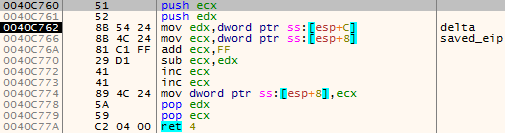
\includegraphics[width=350pt]{obf_func.png}
  \caption{Fonction utilisée pour exécuter une instruction \textit{jmp} de
    manière détournée.}
  \label{fig:func}
\end{figure}

Il y a 11 fonctions comme celle-ci, contenant le même code et qui sont utilisées
à tour de rôle.\\
Dans la figure ci-dessous, la fonction \textit{sage.404924} est une de ces
fonctions.\\

\begin{figure}[H]
  \center
  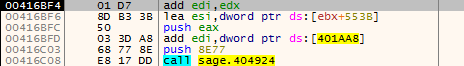
\includegraphics[width=350pt]{obf_usage.png}
  \caption{Utilisation de la fonction pour rendre le flot d'exécution plus
    difficile à suivre.}
  \label{fig:usage}
\end{figure}
\ \\
L'essentiel du code du ransomware est stocké chiffré en mémoire. Le chargement
du code se fait en 2 parties.\\
D'abord, un \textit{stub} (qui est stocké à l'adresse 0x004210BA, chiffré
par des combinaisons de \textit{xor} et de \textit{add})
\footnote{Dans le domaine du packing, un stub est un morceau de code minimal
dont le rôle est de charger une partie plus importante du code qui est chifrée
ou compressée} est déchiffré, copié dans un espace mémoire alloué dynamiquement
puis exécuté.\\
Ce stub se charge ensuite de re-allouer les pages à partir de
l'adresse 0x00400000 (adresse à laquelle est chargée l'image de l'exécutable
en mémoire), supprimant toutes traces des headers et de la section \textit{text}
originale. Il déchiffre ensuite le véritable code du ransomware (qui est
stocké à l'adresse 0x0042166A, chiffré à l'aide de RC4), puis passe
l'exécution au code fraichement déchiffré. Après avoir fait un dump de la partie
packée, on retrouve la véritable liste des fonctions importées ainsi que le
point d'entrée du programme original qui est à l'adresse 0x00406020.\\

\begin{figure}[H]
  \center
  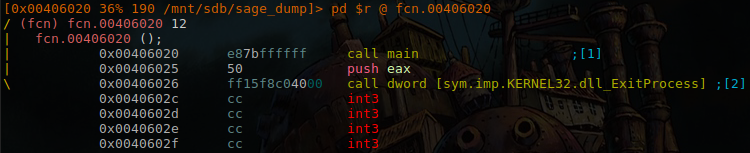
\includegraphics[width=350pt]{oep.png}
  \caption{Point d'entrée du code original, après déchiffrement}
  \label{fig:oep}
\end{figure}

\ \\
Sage n'intègre pas de véritables fonctionnalités d'anti-debug mais tente
simplement de gêner les utilisateurs de débugueurs en simulant un fork au
début de son exécution.
Pour se faire plus discret, Sage tente également de dissimuler sa présence
en faisant une copie de lui-même dans le dossier
\textbf{\%appdata\%\textbackslash Roaming\textbackslash}. Cette copie est nommée
aléatoirement (nom composé de 8 caractères alphanumériques) et c'est elle qui
s'exécute à chaque démarrage de session utilisateur pour assurer la persistance.

\subsection{Main}
Grâce au dump du code original du ransomware, une analyse statique plus
pousée est possible. Bonne nouvelle, la fonction principale est plutôt courte et
sa structure est simple :
\begin{figure}[H]
  \center
  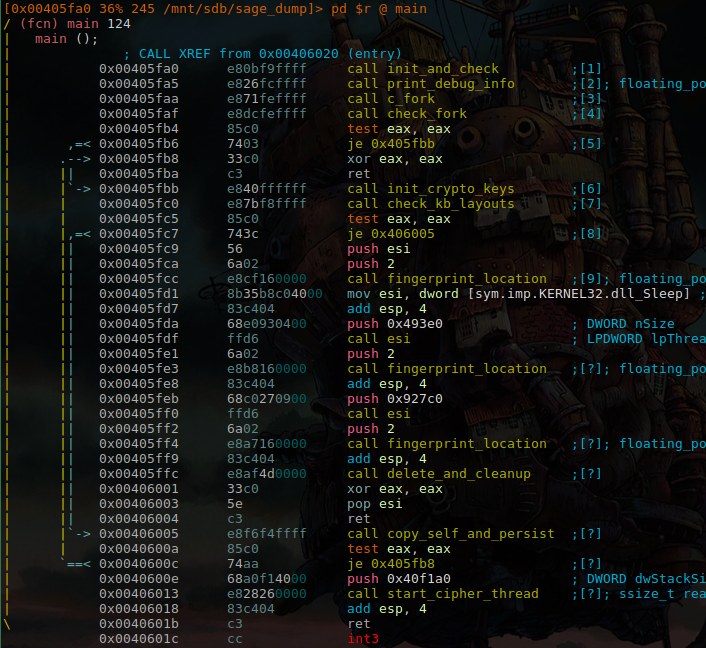
\includegraphics[width=350pt]{main.png}
  \caption{Code assembleur de la fonction principale après déchiffrement}
  \label{fig:main}
\end{figure}

Ce qui donne, en pseudo-code :
\begin{lstlisting}
int main()
{
  init_and_chek();
  print_debug_info();
  c_fork(arg);
  if (check_fork())
    return 0;
  init_crypto_keys();
  if (check_kb_layouts())
  {
    fingerprint_location(2);
    Sleep(0x493E0u);
    fingerprint_location(2);
    Sleep(0x927C0u);
    fingerprint_location(2);
    delete_and_cleanup();
    result = 0;
  }
  else
  {
    if (!copy_self_and_persist())
      return 0;
    result = start_cipher_thread(&encryption_key);
  }
  return result;
}
\end{lstlisting}

\paragraph{Vérification de la langue}
Sage estime la nationalité de la victime, d'après la liste des layouts clavier
utilisés sur la machine, qu'il obtient grâce à la fonction
\textit{GetKeyboardLayoutList}.

\begin{lstlisting}
bool check_kb_layouts()
{
  localeCount = GetKeyboardLayoutList(10, (HKL *)&List);
  if (localeCount <= 0)
    return false;
  i = 0;
  if (localeCount <= 0)
    return false;
  while (true)
  {
    next = (int)(&List)[i] & 0x3FF;
    if (next == 0x23 || next == 0x3F || next == 0x19 || next == 0x22 ||
         next == 0x43 || next == 0x85)
      break;
    if (++i >= localeCount)
      return false;
  }
  return true;
}
\end{lstlisting}
Ces codes correspondent aux layouts clavier suivants :
\begin{itemize}
\item Biélorusse
\item Kazakh
\item Russe
\item Ukrainien
\item Ouzbek
\item Sakha
\end{itemize}
\ \\
Si un de ces layouts clavier est utilisé sur la machine victime, alors Sage
s'arrête avant de chiffrer quoi que ce soit.

\paragraph{Estimation de la localisation}
Si c'est possible (c'est-à-dire, si des bornes Wi-Fi sont détectées), Sage tente
également de localiser plus précisement la machine sur laquelle il s'exécute en
utilisant l'
\href{https://developers.google.com/maps/documentation/geolocation/intro}
{API de géolocalisation Google}.\\
Cette API permet d'estimer la localisation d'une borne Wi-Fi à l'aide de son
adresse MAC et de son SSID.

\paragraph{Persistance}
En ce qui concerne la persistance (l'exécution de lui-même au démarrage),
Sage fait usage des tâches planifiées de Windows. Après s'être copié dans
le dossier \textbf{AppData\textbackslash Roaming\textbackslash}, Sage ajoute une tâche dans la liste
de manière à relancer l'exécution de son binaire à chaque nouvelle connexion
d'un utilisateur sur la machine. Ceci permet de s'assurer que la machine
reste inutilisable après l'infection et ce jusqu'à ce que la rançon
soit payée.\\

\begin{figure}[H]
  \center
  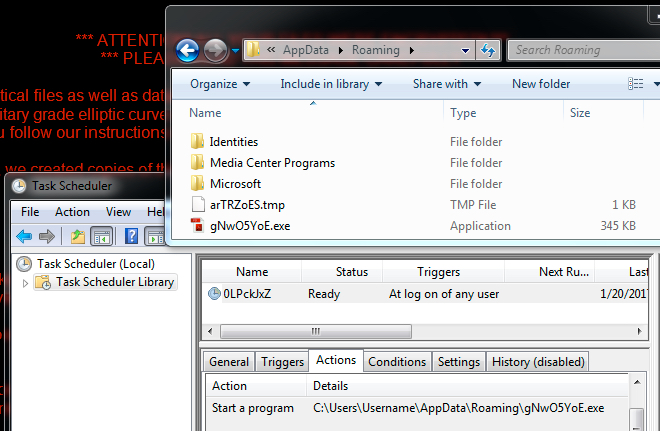
\includegraphics[width=350pt]{persis_task.jpg}
  \caption{Binaire de sage et tâche planifiée utilisée pour maintenir
    l'exécution au démarrage.}
  \label{fig:task}
\end{figure}


\paragraph{Information de debug \& fichier canary}
Certains restes de fonctionnalités de debug sont trouvables dans l'exécutable.
Notamment, la gestion d'un paramètre "d", qui permet d'afficher une information
concernant la configuration du ransomware.

\begin{figure}[H]
  \center
  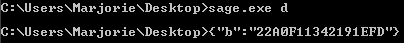
\includegraphics[width=350pt]{debug.jpg}
  \caption{Résultat renvoyé par Sage en lui passant l'argument "d"}
  \label{fig:task}
\end{figure}

Également, vérification de la présence d'un fichier qui permet d'éviter le
lancement du ransomware, certainement utile pour éviter tout lancement
accidentel durant le développement du ransomware :
\begin{lstlisting}
if (CreateFileW(L"C:\\Temp\\lol.txt", 0x80000000, FILE_SHARE_READ, NULL,
     OPEN_EXISTING, 0, NULL) == INVALID_HANDLE_VALUE)
{
	// Chiffrement des fichiers
}
\end{lstlisting}

\paragraph{Communication C\&C}
Sage tente de communiquer à un serveur C\&C durant son exécution. Il essaye
d'abord d'obtenir une adresse IP pour le nom de domaine
\textbf{mbfce24rgn65bx3g.rzunt3u2.com}, et si il n'y parvient pas, envoie
un paquet chiffré à des milliers d'adresses IP différentes en utilisant le
protocole UDP. Le choix du protocole UDP est probablement dû au fait que le
protocole UDP permet d'envoyer un paquet à un serveur sans établir de connexion
ou même attendre de réponse du serveur avec lequel on communique. Cela
permet à Sage de garder la véritable IP du serveur C\&C cachée parmis les
milliers d'IP auxquelles sont envoyés ces paquets.\\

Voici une partie du traffic réseau produit par Sage :
\begin{figure}[H] 
  \center
  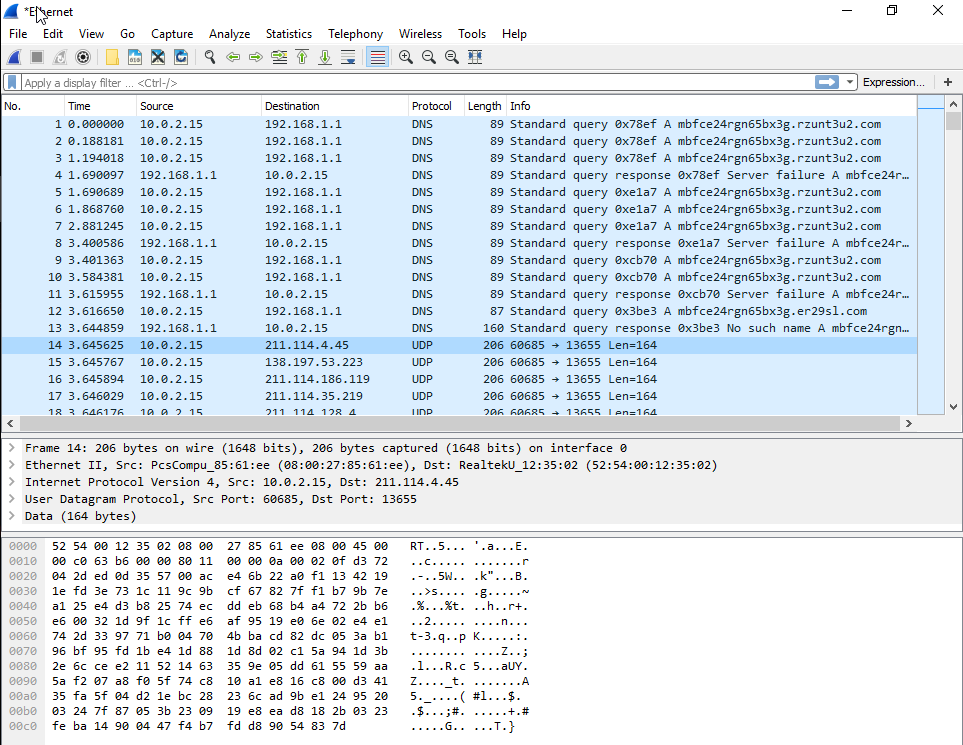
\includegraphics[width=350pt]{packet_log.png}
  \caption{Packets envoyés par Sage lors de son exécution.}
  \label{fig:packets}
\end{figure}

\subsection{Extensions ciblées}
Pour éviter de rendre le système d'exploitation inutilisable en chiffrant des
fichiers critiques, les ransomwares se contentent de chiffrer uniquement les
fichiers dont les noms contiennent les extensions les plus couramment utilisées
pour les fichiers de données utilisateur.\\
En ce qui concerne Sage, cette liste est la suivante :
\begin{lstlisting}
.dat .mx0 .cd .pdb .xqx .old .cnt .rtp .qss .qst .fx0 .fx1 .ipg .ert .pic .img
.cur .fxr .slk .m4u .mpe .mov .wmv .mpg .vob .mpeg .3g2 .m4v .avi .mp4 .flv
.mkv .3gp .asf .m3u .m3u8 .wav .mp3 .m4a .m .rm .flac .mp2 .mpa .aac .wma .djv
.pdf .djvu .jpeg .jpg .bmp .png .jp2 .lz .rz .zipx .gz .bz2 .s7z .tar .7z .tgz
.rar .zip .arc .paq .bak .set .back .std .vmx .vmdk .vdi .qcow .ini .accd .db
.sqli .sdf .mdf .myd .frm .odb .myi .dbf .indb .mdb .ibd .sql .cgn .dcr .fpx
.pcx .rif .tga .wpg .wi .wmf .tif .xcf .tiff .xpm .nef .orf .ra .bay .pcd .dng
.ptx .r3d .raf .rw2 .rwl .kdc .yuv .sr2 .srf .dip .x3f .mef .raw .log .odg .uop
.potx .potm .pptx .rss .pptm .aaf .xla .sxd .pot .eps .as3 .pns .wpd .wps .msg
.pps .xlam .xll .ost .sti .sxi .otp .odp .wks .vcf .xltx .xltm .xlsx .xlsm
.xlsb .cntk .xlw .xlt .xlm .xlc .dif .sxc .vsd .ots .prn .ods .hwp .dotm .dotx
.docm .docx .dot .cal .shw .sldm .txt .csv .mac .met .wk3 .wk4 .uot .rtf .sldx
.xls .ppt .stw .sxw .dtd .eml .ott .odt .doc .odm .ppsm .xlr .odc .xlk .ppsx
.obi .ppam .text .docb .wb2 .mda .wk1 .sxm .otg .oab .cmd .bat .h .asx .lua .pl
.as .hpp .clas .js .fla .py .rb .jsp .cs .c .jar .java .asp .vb .vbs .asm .pas
.cpp .xml .php .plb .asc .lay6 .pp4 .pp5 .ppf .pat .sct .ms11 .lay .iff .ldf
.tbk .swf .brd .css .dxf .dds .efx .sch .dch .ses .mml .fon .gif .psd .html
.ico .ipe .dwg .jng .cdr .aep .aepx .123 .prel .prpr .aet .fim .pfb .ppj .indd
.mhtm .cmx .cpt .csl .indl .dsf .ds4 .drw .indt .pdd .per .lcd .pct .prf .pst
.inx .plt .idml .pmd .psp .ttf .3dm .ai .3ds .ps .cpx .str .cgm .clk .cdx .xhtm
.cdt .fmv .aes .gem .max .svg .mid .iif .nd .2017 .tt20 .qsm .2015 .2014 .2013
.aif .qbw .qbb .qbm .ptb .qbi .qbr .2012 .des .v30 .qbo .stc .lgb .qwc .qbp
.qba .tlg .qbx .qby .1pa .ach .qpd .gdb .tax .qif .t14 .qdf .ofx .qfx .t13 .ebc
.ebq .2016 .tax2 .mye .myox .ets .tt14 .epb .500 .txf .t15 .t11 .gpc .qtx .itf
.tt13 .t10 .qsd .iban .ofc .bc9 .mny .13t .qxf .amj .m14 ._vc .tbp .qbk .aci
.npc .qbmb .sba .cfp .nv2 .tfx .n43 .let .tt12 .210 .dac .slp .qb20 .saj .zdb
.tt15 .ssg .t09 .epa .qch .pd6 .rdy .sic .ta1 .lmr .pr5 .op .sdy .brw .vnd .esv
.kd3 .vmb .qph .t08 .qel .m12 .pvc .q43 .etq .u12 .hsr .ati .t00 .mmw .bd2 .ac2
.qpb .tt11 .zix .ec8 .nv .lid .qmtf .hif .lld .quic .mbsb .nl2 .qml .wac .cf8
.vbpf .m10 .qix .t04 .qpg .quo .ptdb .gto .pr0 .vdf .q01 .fcr .gnc .ldc .t05
.t06 .tom .tt10 .qb1 .t01 .rpf .t02 .tax1 .1pe .skg .pls .t03 .xaa .dgc .mnp
.qdt .mn8 .ptk .t07 .chg .#vc .qfi .acc .m11 .kb7 .q09 .esk .09i .cpw .sbf .mql
.dxi .kmo .md .u11 .oet .ta8 .efs .h12 .mne .ebd .fef .qpi .mn5 .exp .m16 .09t
.00c .qmt .cfdi .u10 .s12 .qme .int? .cf9 .ta5 .u08 .mmb .qnx .q07 .tb2 .say
.ab4 .pma .defx .tkr .q06 .tpl .ta2 .qob .m15 .fca .eqb .q00 .mn4 .lhr .t99
.mn9 .qem .scd .mwi .mrq .q98 .i2b .mn6 .q08 .kmy .bk2 .stm .mn1 .bc8 .pfd .bgt
.hts .tax0 .cb .resx .mn7 .08i .mn3 .ch .meta .07i .rcs .dtl .ta9 .mem .seam
.btif .11t .efsl .$ac .emp .imp .fxw .sbc .bpw .mlb .10t .fa1 .saf .trm .fa2
.pr2 .xeq .sbd .fcpa .ta6 .tdr .acm .lin .dsb .vyp .emd .pr1 .mn2 .bpf .mws
.h11 .pr3 .gsb .mlc .nni .cus .ldr .ta4 .inv .omf .reb .qdfx .pg .coa .rec .rda
.ffd .ml2 .ddd .ess .qbmd .afm .d07 .vyr .acr .dtau .ml9 .bd3 .pcif .cat .h10
.ent .fyc .p08 .jsd .zka .hbk .mone .pr4 .qw5 .cdf .gfi .cht .por .qbz .ens
.3pe .pxa .intu .trn .3me .07g .jsda .2011 .fcpr .qwmo .t12 .pfx .p7b .der .nap
.p12 .p7c .crt .csr .pem .gpg .key
\end{lstlisting}

\subsection{Chiffrement}
Sage se démarque des autres ransomwares en ce qui concerne le chiffrement
puisqu'il fait usage de cryptographie sur les courbes elliptiques ainsi que
de l'algorithme ChaCha pour chiffrer les fichiers de l'utilisateur, ce qui
n'est pas commun.\\
ChaCha est un algortihme de chiffrement à flot dérivé de Salsa20; Sage l'utilise
pour chiffrer le contenu des fichiers.\\
Chaque fichier cible est renommé et chiffré avec une clé ChaCha
choisie aléatoirement, et cette clé est ensuite stockée à la fin du fichier
chiffré. Cette clé n'est évidemment pas stockée tel quel dans le fichier, ce
sont en fait deux parties qui permettent, si on possède une valeur secrète, de
retrouver la clé utilisée pour chiffrer le fichier, qui sont stockées.\\
Il est important de noter que Sage prend soin de supprimer les sauvegardes
de fichiers faites avec \textit{Shadow Copy} avant de commencer le chiffrement.
\ \\
Les calculs sont faits sur la courbe elliptique \textit{Curve25519} (d'équation
$y^2 = x^3 + 486662*x^2 + x$, sur $\mathbb{F}_p = GF(2^{255} - 19)$), qui est
une courbe populaire pour plusieurs raisons (sécurité, rapidité des calculs,
propriétés liées à la génération d'éléments aléatoires) et qui est conçue pour
être utilisée par le protocole ECDH (Elliptic Curve Diffie-Hellman).\\
Dans la suite, on notera $\mathbb{F}_p = GF(2^{255} - 19)$ et $G$ le point de
la courbe $Curve25519$ admettant $x = 9$. Enfin, le ransomware a connaissance de
$Q_s = k_s * G$, la partie publique de l'extorqueur utilisée lors de la création
du secret partagé.\\
Le chiffrement d'un fichier se déroule comme ceci :
\begin{itemize}
\item On génère $k_c \in \mathbb{F}_p$ aléatoirement
\item On calcule le point $Q_c = k_c * G$
\item On calcule le secret partagé $S = k_c * Q_s = (k_c * k_s) * G$
\item On dérive du secret partagé, un entier $sh \in \mathbb{F}_p$
\item On calcule le point $P = sh * G$
\item On génère $n \in \mathbb{F}_p$ aléatoirement
\item On calcule les points $chacha\_key = n * P = (n * sh) * G$ et
  $chacha\_pub = n * G$
\item On chiffre le fichier en utilisant ChaCha avec une clé dérivée de
  $chacha\_key$ 
\item On ajoute les valeurs de $Q_c$ et $chacha\_pub$ à la fin du fichier
\end{itemize}
\ \\

Ce qui produit, en pratique, un fichier de la forme :
\begin{figure}[H]
  \center
  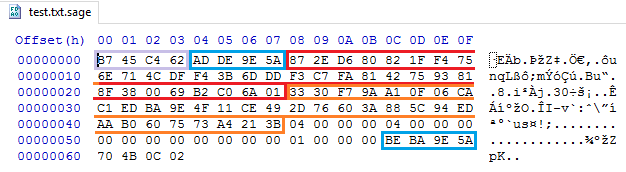
\includegraphics[width=350pt]{dump_file.png}
  \caption{Contenu d'un fichier après avoir été chiffré par Sage.}
  \label{fig:file}
\end{figure}
\ \\
Légende :
\begin{itemize}
\item Mauve : Contenu chiffré du fichier original
\item Rouge : $Q_c$
\item Orange : $chacha\_pub$
\item Bleu : Valeurs constantes
\end{itemize}

Petite note sur le déchiffrement; il est nécéssaire de connaître la valeur
de $k_s$ pour pouvoir déchiffrer les fichiers. Cette valeur n'est stockée
nulle part dans le binaire et on peut donc supposer que seul l'auteur du
ransomware la possède, évidemment. Étant donné qu'il n'est donc pas possible,
en pratique, de calculer $k_s$ en un temps raisonnable, le seul moyen de
déchiffrer les fichiers est donc, soit de payer, soit d'attendre que la clé
privée fuite ou soit retrouvée sur des serveurs saisis par la police (comme ce
fut le cas pour le ransomware ICEPOL).\\
Le déchiffrement d'un fichier se déroule comme ceci :
\begin{itemize}
\item On récupère les valeurs $Q_c$ et $chacha\_pub$
\item On calcule le secret partagé $S = k_s * Q_c = (k_s * k_c) * G$
\item On dérive du secret partagé, l'entier $sh \in \mathbb{F}_p$
\item On calcule le point $chacha\_key = sh * chacha\_pub = (sh * n) * G$
\item On déchiffre le fichier en utilisant ChaCha avec la clé dérivée
  de $chacha\_key$
\end{itemize}
